\documentclass{article}

\usepackage[utf8]{inputenc}
\usepackage[brazil]{babel}
\usepackage{amsmath, amssymb}
\usepackage{graphicx}
\usepackage{hyperref}
\usepackage{float}
\usepackage{geometry}
\usepackage{caption}
\usepackage{listings}
\usepackage{color}
\usepackage{courier}

\geometry{margin=1in}

\title{Variáveis Instrumentais}
\author{Eduardo Henrique Basilio de Carvalho}
\date{\today}

\begin{document}

\maketitle

\section*{Questão 1}

A figura \ref{fig:armax_histogramas} mostra os histogramas dos coeficientes estimados pelos métodos MQ e VI para o modelo ARMAX.

\begin{figure}[H]
    \centering
    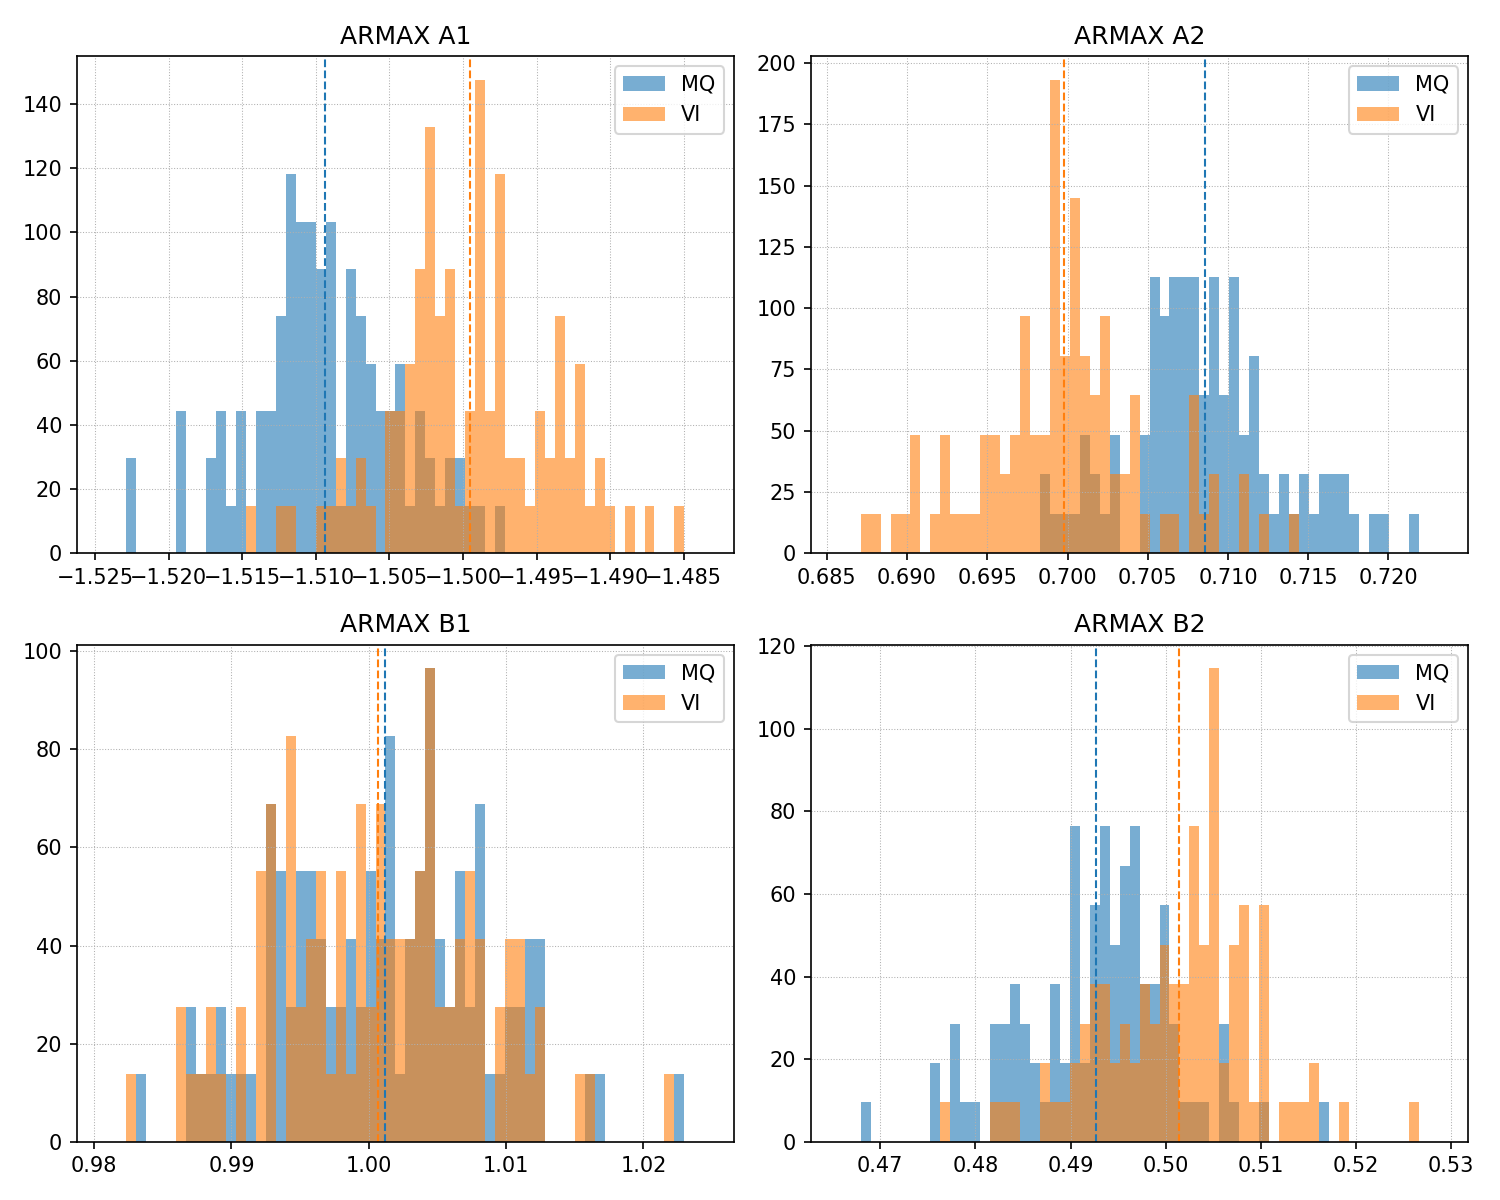
\includegraphics[width=\textwidth]{imagens/armax_histogramas.png}
    \caption{Histogramas dos coeficientes estimados pelos métodos MQ e VI para o modelo ARMAX.}
    \label{fig:armax_histogramas}
\end{figure}

Para os coeficientes A1, A2 e B2, VI apresenta viés muito inferior ao MQ e uma variância similar. Já para o coeficiente B1, ambos os métodos apresentam viés similar e baixa, com variança também similar.

A figura \ref{fig:oe_histogramas} os histogramas dos coeficientes estimados pelos métodos MQ e VI para o modelo OE.

\begin{figure}[H]
    \centering
    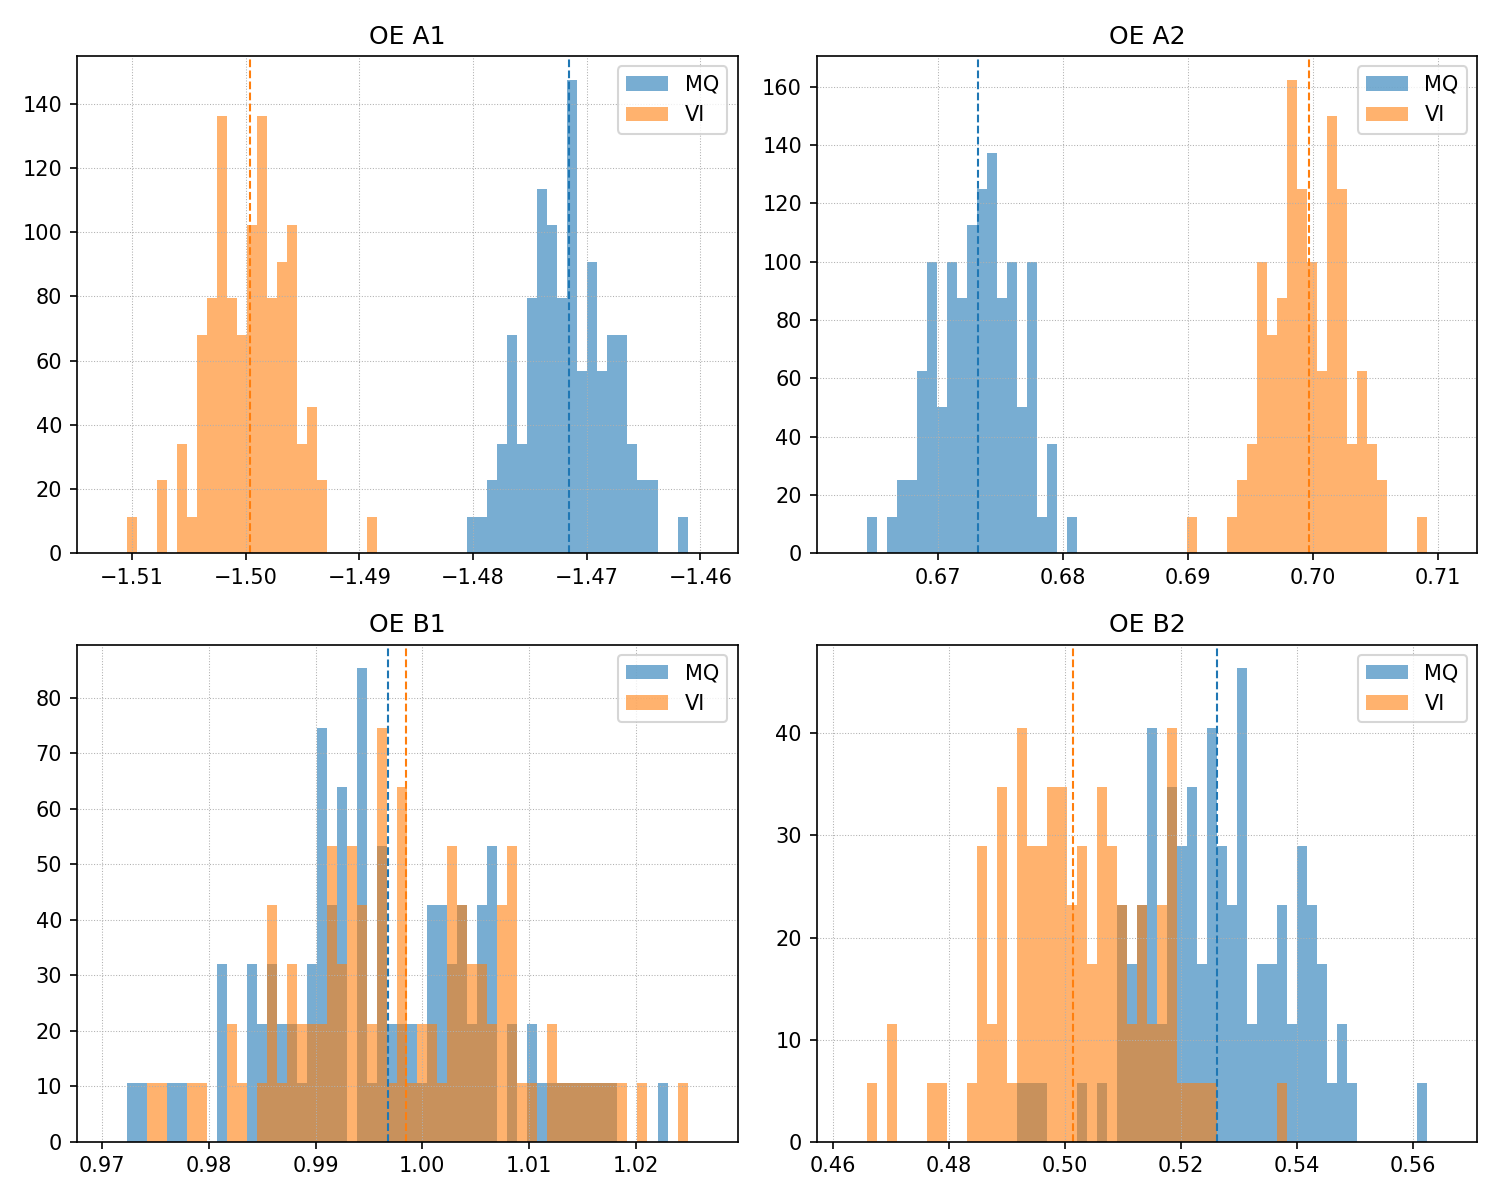
\includegraphics[width=\textwidth]{imagens/oe_histogramas.png}
    \caption{Histogramas dos coeficientes estimados pelos métodos MQ e VI para o modelo OE.}
    \label{fig:oe_histogramas}
\end{figure}

Neste caso, a diferença entre os métodos é ainda mais pronunciada. Para todos os coeficientes, VI apresenta viés inferior ao MQ, com variância similar.

\section*{Questão 2}

A figura \ref{fig:ararx_histogramas} mostra os histogramas dos coeficientes estimados pelos métodos EMQ, GMQ e VI para o modelo ARARX.

\begin{figure}[H]
    \centering
    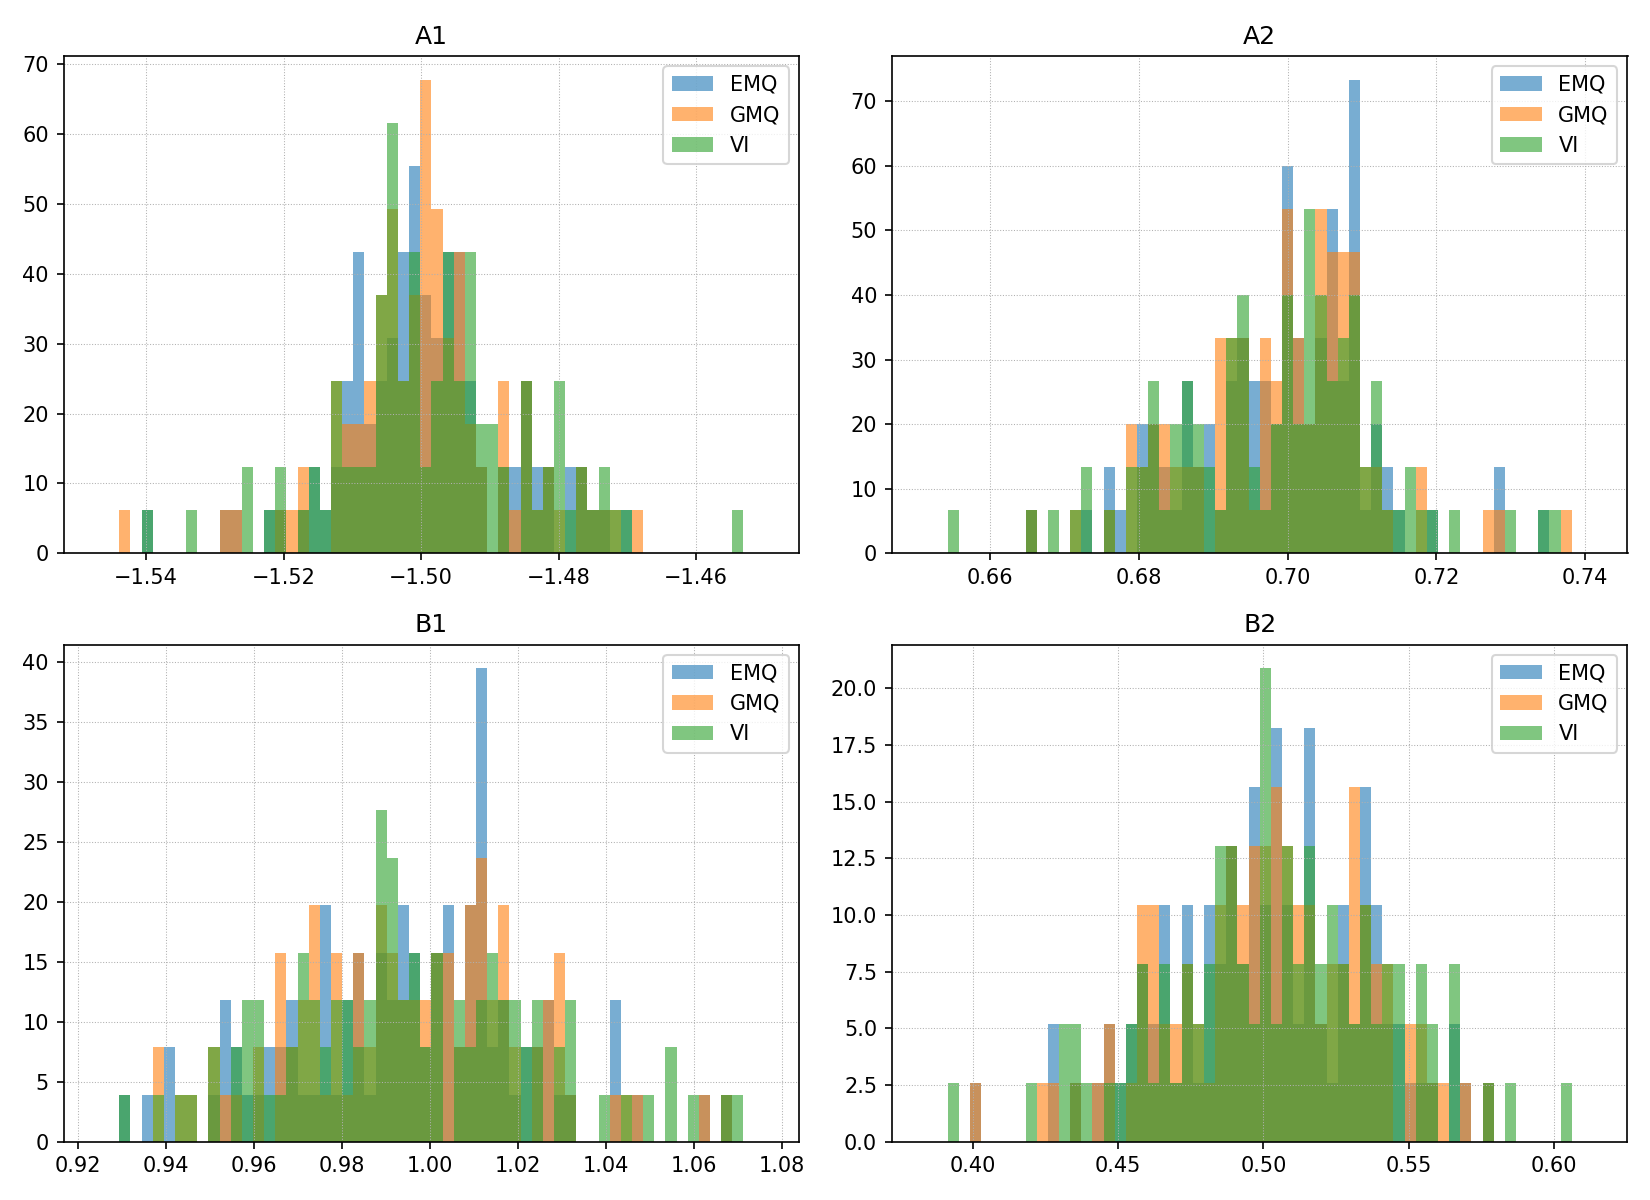
\includegraphics[width=\textwidth]{imagens/ararx_histogramas.png}
    \caption{Histogramas dos coeficientes estimados pelos métodos EMQ, GMQ e VI para o modelo ARARX.}
    \label{fig:ararx_histogramas}
\end{figure}

O modelo é simulado na função \ref{code:simulate_generator}. Os estimadores EMQ, GMQ e VI são implementados nas funções \ref{code:estimate_els}, \ref{code:estimate_gls_with_true_filter} e \ref{code:estimate_arx_iv}, respectivamente.

\begin{lstlisting}[language=Python, caption={Simula o gerador do sistema.}, label={code:simulate_generator}, basicstyle=\ttfamily\footnotesize, breaklines=true]
def simulate_generator(A: np.ndarray, B: np.ndarray, nk: int, u: np.ndarray, w: np.ndarray, H_alpha: float):
    N = u.size
    na = A.size
    nb = B.size
    y = np.zeros(N)
    e = np.zeros(N)
    for k in range(N):
        
        ar_part = 0.0
        for i in range(1, na + 1):
            ar_part -= A[i - 1] * safe_get(y, k - i)
        in_part = 0.0

        for j in range(1, nb + 1):
            in_part += B[j - 1] * safe_get(u, k - nk - (j - 1))

        e[k] = safe_get(w, k) - H_alpha * safe_get(e, k - 1)

        y[k] = ar_part + in_part + e[k]
    return y
\end{lstlisting}

\begin{lstlisting}[language=Python, caption={Estimador Estendido de Mínimos Quadrados (EMQ).}, label={code:estimate_els}, basicstyle=\ttfamily\footnotesize, breaklines=true]
def estimate_els(y: np.ndarray, u: np.ndarray, na: int, nb: int, nk: int, n_iter: int = 6):
    theta = np.zeros(na + nb)
    A_ls, B_ls = estimate_arx_ls(y, u, na, nb, nk)
    theta[:na] = A_ls
    theta[na:] = B_ls
    N = y.size
    for _ in range(n_iter):
        Phi, Y, _ = build_regression(y, u, na, nb, nk)
        res = Y - (Phi @ theta)
        if res.size < 2:
            alpha = 0.0
        else:
            num = np.dot(res[1:], res[:-1])
            den = np.dot(res[:-1], res[:-1])
            s = num / den if den != 0 else 0.0
            alpha = -s
        y_pref = prefilter_sequence(y, alpha)
        u_pref = prefilter_sequence(u, alpha)
        Phi_pref, Y_pref, _ = build_regression(y_pref, u_pref, na, nb, nk)
        theta = np.linalg.pinv(Phi_pref) @ Y_pref
    return theta[:na].copy(), theta[na:].copy()
\end{lstlisting}

\begin{lstlisting}[language=Python, caption={Estimador Generalizado de Mínimos Quadrados (GMQ) com o filtro verdadeiro.}, label={code:estimate_gls_with_true_filter}, basicstyle=\ttfamily\footnotesize, breaklines=true]
def estimate_gls_with_true_filter(y: np.ndarray, u: np.ndarray, na: int, nb: int, nk: int, true_alpha: float):
    y_pref = prefilter_sequence(y, true_alpha)
    u_pref = prefilter_sequence(u, true_alpha)
    Phi_pref, Y_pref, _ = build_regression(y_pref, u_pref, na, nb, nk)
    theta = np.linalg.pinv(Phi_pref) @ Y_pref
    return theta[:na].copy(), theta[na:].copy()
\end{lstlisting}

\begin{lstlisting}[language=Python, caption={Estimador de Variáveis Instrumentais (VI).}, label={code:estimate_arx_iv}, basicstyle=\ttfamily\footnotesize, breaklines=true]
def iterative_iv(y: np.ndarray, u: np.ndarray, na: int, nb: int, nk: int, n_iter: int = 8):
    Phi, Y, start = build_regression(y, u, na, nb, nk)
    theta = np.linalg.pinv(Phi) @ Y
    N = y.size
    for _ in range(n_iter):
        y_sim = simulate_arx(theta, u, na, nb, nk)
        M = Phi.shape[0]
        Z = np.zeros_like(Phi)
        for idx, k in enumerate(range(start, N)):
            for i in range(1, na + 1):
                Z[idx, i - 1] = -safe_get(y_sim, k - i)
            for j in range(1, nb + 1):
                Z[idx, na + j - 1] = safe_get(u, k - nk - (j - 1))
        ZtPhi = Z.T @ Phi
        theta = np.linalg.pinv(ZtPhi) @ (Z.T @ Y)
    return theta[:na].copy(), theta[na:].copy()
\end{lstlisting}

Naqueles em que o erro é modelado, a função \ref{code:prefilter_sequence} é utilizada como implementação da respectiva regressora.

\begin{lstlisting}[language=Python, caption={Pré-filtro para o ruído AR(1).}, label={code:prefilter_sequence}, basicstyle=\ttfamily\footnotesize, breaklines=true]
def prefilter_sequence(x: np.ndarray, alpha: float):
    N = x.size
    x_pref = np.zeros(N)
    for k in range(N):
        x_pref[k] = x[k] + alpha * safe_get(x_pref, k - 1)
    return x_pref
\end{lstlisting}

Mesmo com poucas amostras (N = 100) e iterações (4), todos os estimadores conseguem desempenho razoável e similar.

\end{document}
